
     The design of the tube is driven by the configuration of the pod.
     Consequently, the system model is constructed such that the pod design is analyzed first.
     The Pod group contains all subsystems onboard the passenger pod.
     The Pod module takes in design variables and feeds them into the Drag, Cycle,
     Drivetrain, Geometry, Mass, and Levitation subsystems.

  \subsubsection{Drag}
    Computational Fluid Dynamics (CFD) was performed on the pod to determine
    how the pod drag coefficient varies with Mach number.
    Pod aerodynamics were computed with the Fully Unstructured Navier-Stokes 3D
    (FUN3D) flow solver \cite{Biedron}. FUN3D is a node-based computational fluid dynamics
    code for mixed element types that uses a second-order accurate point-implicit
    method for numerical convergence. The upwind inviscid flux difference
    splitting scheme of Roe \cite{Roe} was used to compute cell interface fluxes,
    with turbulence closure obtained using the one equation model of Spalart
    and Allmaras \cite{Spalart}.
    All computational boundaries were discretized using the Glyph scripting
    language of the commercial mesh software Pointwise®. Volume discretizations
    were generated from the surface domains using the advancing-front local
    reconnection (AFLR3)\cite{Marcum} algorithm. For computational efficiency, extruded
    viscous prism layers were generated near the pod surfaces and transitioned
    to isotropic tetrahedral cells outside the boundary layer region.
    All viscous cells were resolved to a $y^{+} < 1$. Volume meshes for the core
    domain contained approximately 19 million cells.

    The computational domain is depicted in \Cref{fig:CFDmodel},
    and modeled assuming vehicle half-symmetry.
    The tube was simulated thirty vehicle body lengths upstream of the pod
    and extended one hundred body lengths downstream. Boundary conditions were
    applied on all computational domains. A freestream condition enforcing Mach
    number and static air reference properties was specified at the tube inflow boundary.
    A uniform static backpressure was specified on the tube downstream exit.
    An inviscid boundary condition was prescribed on the tube walls to avoid
    the formation of a viscous boundary layer. All surfaces of the pod were
    assigned a viscous no-slip condition, except flow-through domains where
    compressor and nozzle boundary conditions were applied. At the compressor
    fan face, a uniform static back-pressure was prescribed. At the nozzle plenum,
    total temperature and pressure ratios with respect to freestream were specified.

    Drag coefficients, non-dimensionalized by pod planform area,
    were extracted from simulation results.
    Drag forces included only viscous and pressure forces acting on external
    pod surfaces and excluded ram and internal nozzle drag effects.

    \begin{figure}
      \centering
      \begin{subfigure}[t]{.5\textwidth}
        \centering
        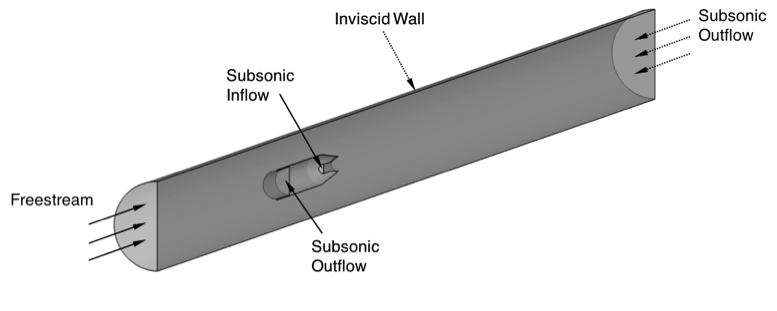
\includegraphics{../../images/CFDmodel.png}
        \caption{Computational boundary applied to vehicle flow domain.}
        \label{fig:CFDmodel}
      \end{subfigure}%
      \begin{subfigure}[t]{.5\textwidth}
        \centering
        \includegraphics[width=.75\textwidth]{../../images/hyperloopIsoView.png}
        \caption{Resulting Flow Contour}
      \label{fig:CFDresults}
      \end{subfigure}
      \caption{CFD model}
      \label{fig:CFD}
    \end{figure}

    % \begin{figure}
    % 	\centering
    % 	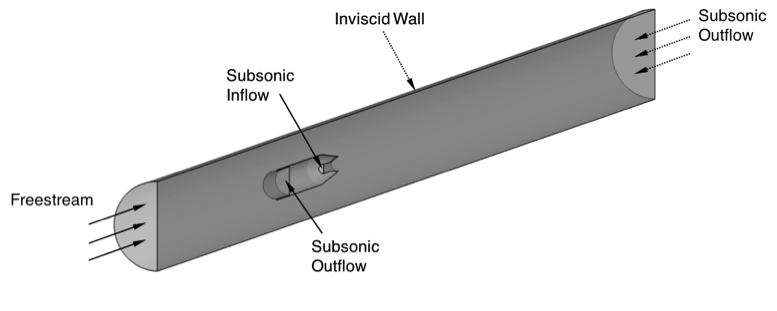
\includegraphics[width=.75\textwidth]{../../images/CFDmodel.png}
    % 	\caption{Computational boundary conditions applied to hyperloop flow domain.}
    % 	\label{fig:CFDmodel}
    % \end{figure}

    \begin{figure}
      \centering
      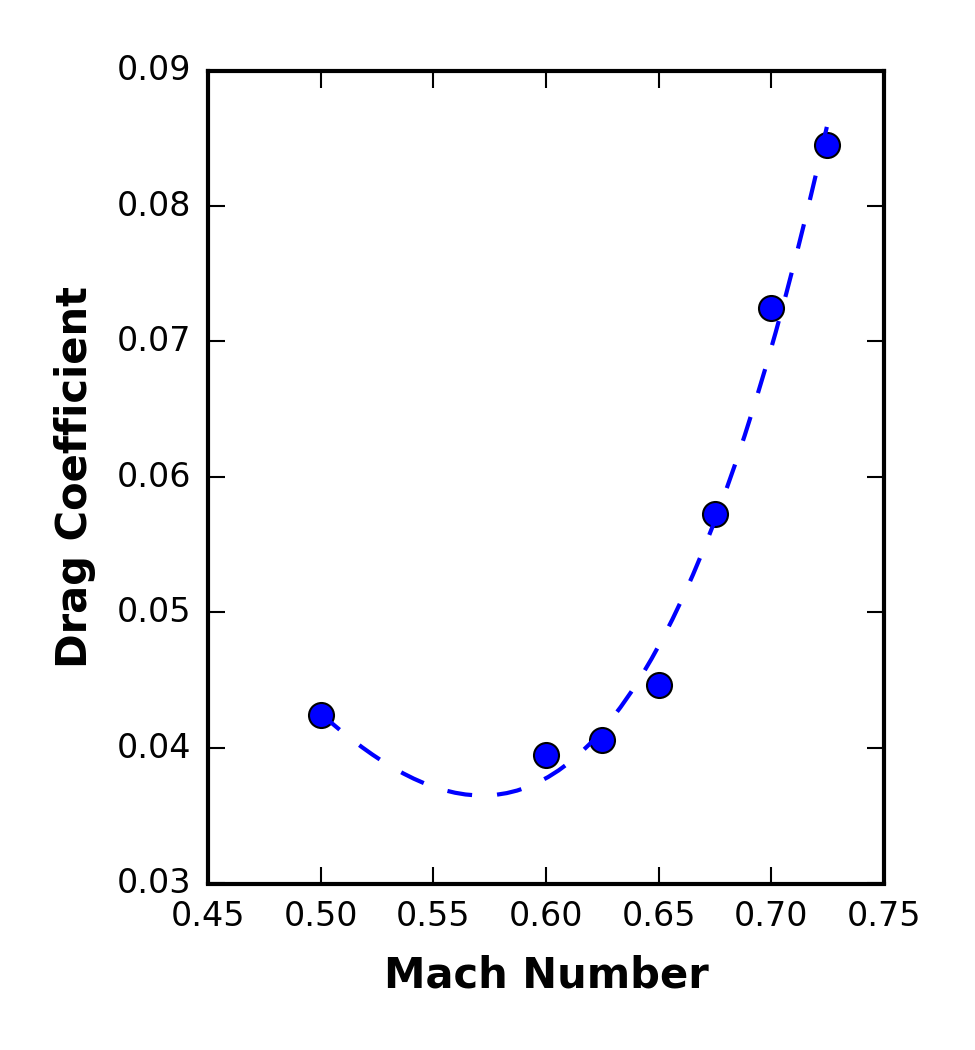
\includegraphics{../../images/graphs/cd_vs_mach/cd_vs_mach.png}
      \caption{Drag Coefficient vs. Mach Number}
      \label{fig:cd_vs_mach}
    \end{figure}
    \Cref{fig:cd_vs_mach} shows the CFD results for drag coefficient vs. Mach number.
    These results fit the trend expected for transonic flow given by the
    Prandtl-Glauert relationship. Drag coefficient values will be interpolated
    from this data for each Mach number the system analyzes.
  \subsubsection{Cycle}
    The on-board compression system provides a means of increasing the maximum
    pod speed over a closed pod,  and provides a small amount of thrust.
    A thermodynamic analysis of the compressor system is necessary to estimate
    on-board power requirements and overall heat rise of each pod.
    The compression cycle is comprised of an inlet, compressor, duct, nozzle,
    and shaft that is connected to the electric motor drivetrain. The design
    deviates from the original Hyperloop proposal by removing two heat
    exchangers as well as the air-bearings. The system is modeled as a
    one-dimensional cycle, representing components as thermodynamic processes
    that are subsequently chained together. Each component is responsible for
    calculating gas properties across its boundaries and appropriately enforcing
    conservation equations across the entire system. This model builds off the
    NASA Glenn developed PyCycle framework, which is a thermodynamic modeling
    framework developed in Python with the capability for optimization
    employing analytic gradients. \cite{PyCycle}
  \subsubsection{Drivetrain}
    The Drivetrain module models an electric motor, inverter, and battery system by
    computing the size and mass of both the motor and battery system
	required to sustain the torque and power demands
	over a mission profile \cite{GeorgiaTechMotor, NASASugar}. The model
	modifies an existing algorithm developed at NASA for battery sizing by utilizing
  a spline fit of voltage discharge curves provided by battery manufacturers
  to compute voltage as a function of discharge instead of the generic physics-based
  model used in previous work \cite{NASASugar}.
  This change provides results that are more flexible and specific to the
	leading commercial battery cells.
\subsubsection{Geometry and Mass}
	In order to analyze the design of the tube structure, the final mass and
	geometric configuration of the pod must be obtained. The Geometry model
	assumes the pod to have a cylindrical fuselage with conical frustums at
	the inlet and exit. The cross sectional area of the passenger section
	given by the user is added to the cross sectional area of the compressor
	exit duct, which is computed in the cycle analysis. The Geometry module
	also estimates the thickness of the pod wall and the passenger compartment
	based on simple pressurized cylinder relationships. It then adds these areas
	together to compute the total cross sectional area. The length of each
	component is also fed into the Geometry model so it can compute the total
	pod length and planform area. The Mass module takes the mass of each
	component and adds them with the total passenger mass in order to determine
	the mass of the pod, without magnets, for levitation. The Levitation component
	takes in this mass, computes the mass of the magnets, then outputs the total mass of the pods.
\subsubsection{Pod Mach}
	The Pod Mach module uses the pod cross-sectional area, Mach number, and
	compressor inlet conditions to compute the tube area. As the pod travels,
	flow that is not entrained by the compressor must accelerate around the pod.
	Due to the pod’s transonic flight speed, it is possible that this bypass
	flow could accelerate to Mach 1 and cause the flow to choke, which would
	lead to an undesirable buildup of pressure in front of the pod and
	increased drag. To avoid this condition, this module sizes the tube area
	such that there is a large enough bypass area to prevent the bypass flow
	from accelerating to Mach 1. This is done using a simple quasi 1D area
	relationship for compressible flow given by the equation
	\begin{equation}
		\label{eq:mach_to_area}
		\frac{A_{1}}{A_{2}}=\frac{M_{2}}{M_{1}} \left( \frac{1+\frac{\gamma -1}{2}M_{1}^{2}}{1+\frac{\gamma -1}{2}M_{2}^{2}} \right)^{\frac{( \gamma +1 )}{2 ( \gamma -1  )}}
	\end{equation}
	For this analysis, $M_1$ is the free stream Mach number, $M_2$ is the
	desired bypass Mach number, $A_1$ is the initial area of the bypass flow
	($A_{tube}$ - $A_{inlet}$), and $A_2$ is the bypass area ($A_{tube}$ - $A_{pod}$).
	For these analyses, $M_2$ is set to .95 in order to provide a slight factor
	of safety to prevent the flow from reaching the choking condition.
	In order to make this model higher fidelity, it is possible to modify the
	areas in the relationship to account for boundary layer development over
	the pod's outer surface. As the boundary develops, the effective bypass area
	is reduced which increases the risk of bypass flow reaching Mach 1. However,
	it is possible to modify this by increasing the effective pod radius by the
	displacement thickness of the boundary layer. The sensitivity of structural
	design to boundary layer growth is important and will be discussed at length later.
\subsubsection{Levitation}

	The Hyperloop concept operates using a levitation system to significantly
	reduce friction during high velocity travel. In this analysis, a
	passive magnetic levitation system is used to suspend the pod above the
	track. A passive system is advantageous because it requires
	zero power input for levitation to occur. The Halbach array passive levitation method
	developed at the Lawrence Livermore National Laboratory is chosen as the
	system for our Hyperloop model \cite{inductrack}. It is assumed that
	ferrite tiles were not used so that the added inductive loading is set to
	zero, leaving only the distributed inductance to compute in the model.
	Fringe fields from the magnetic array are also ignored in this analysis and
	the width of the magnetic array is set equal to the width of the track.
	These three simplifications and assumptions allow the overall scale factor
	for the total force, $levsf$, to be set equal to unity.

	The Levitation group makes two critical calculations: the inductance of the
	track required for the pod to levitate at a desired speed and the mass of
	the permanent magnets located onboard. The Breakpoint Levitation module employs a
	desired minimum levitation speed and uses it to calculate important track
	parameters, including the ratio of inductance to resistance of the track.

	Using the desired levitation speed, the total mass of magnets required and
	drag force produced is then calculated. The lift and drag produced
	by the magnets are given by \cref{eq:fy_lev} and \cref{eq:dmag}
	\begin{equation}
		\label{eq:fy_lev}
		L_{mag} = F_{y}(\omega)=\frac{\beta _{0}^{2}w_{mag}\lambda}{4\pi Ld_{c}}\frac{1}{(1+R/\omega L)^{2}}A_ae^{-4\pi h/\lambda } \ ,
	\end{equation}
	%Fyuf equations from http://cegt201.bradley.edu/projects/proj2004/maglevt1/Inductrack1.m
	\begin{equation}
		\label{eq:dmag}
		D_{mag}=( m_{pod}g)R/\omega L
	\end{equation}
	In these equations, the drag and the magnet mass are both functions of the
	magnet area and thickness. To minimize drag and mass, a Pareto optimization
	is performed prior to running the system model. The following cost function
	is developed by normalizing drag and mass, then multiplying by a weighting
	factor $alpha$ and adding them together in the following equation
	\begin{equation}
		\label{eq:pareto}
		f(\alpha ) = \alpha \bar{F_{x}} + (1-\alpha )\bar{m_{mag}}v
	\end{equation}
	Where the bar signifies the normalized value. The weighting factor $alpha$
	is chosen arbitrarily between zero and unity; high values of $alpha$
	emphasize minimizing drag while low values of $alpha$ emphasize minimizing mass.




